\subsubsection{Einstellen von Wirk- und Blindleistung}
Bei dieser Messung wurde die Wirk- bzw. Blindleistung anhand des Zündwinkels und der DC-Spannung (Zündwinkel $\theta = 0°$) eingestellt. \\

Für den Effektivwert wurde die Wirk- bzw. Blindleistung folgendermassen ausgerechnet. \\
$S = U*I, U=const$
P abgelesen
$Q = \sqrt{(S^2 - P^2)}$
\begin{figure}[!ht]
  \begin{center}
  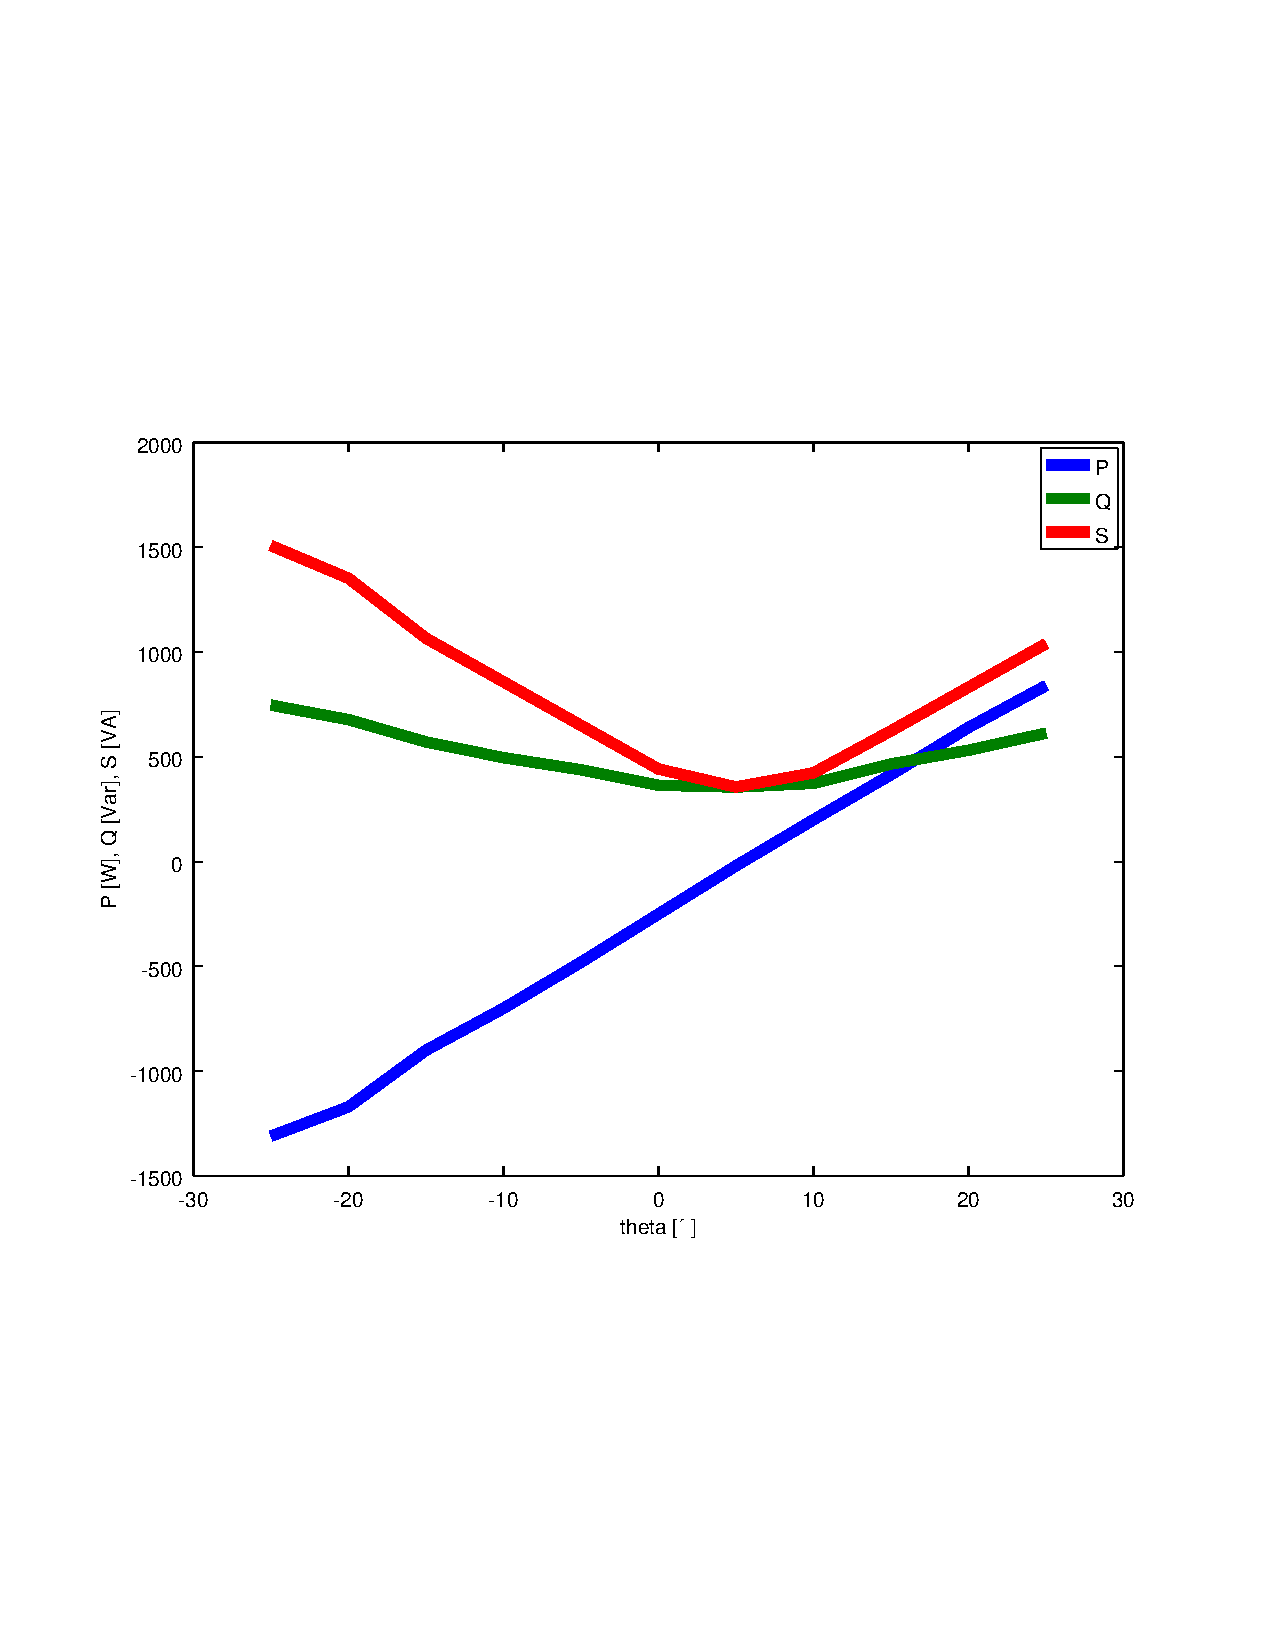
\includegraphics[width=0.5\textwidth, trim={1cm 6.5cm 2cm 7cm},clip]{pic/6_1_grundfrequenztaktung/6_1_2_einst_wirk_und_blindleistung/P_Q_S.pdf}
  \caption{$P(\theta) (blau), Q(\theta) (grün), S(\theta) (rot)$ von dem Effektivwert in Abhängigkeit des Zündwinkels}
  \label{fig:6_1_2_0}
  \end{center}
\end{figure}


Für die Grundschwingung wurde die Wirk- bzw. Blindleistung folgendermassen ausgerechnet.\\
$S_1 = U_1 * I_1$
\underline{I1} abgelesen, Trigger auf Strom
$P_1 = S_1 * cos(\phi)$
$Q_1 = S_1 * sin(\phi)$
\begin{figure}[!ht]
  \begin{center}
  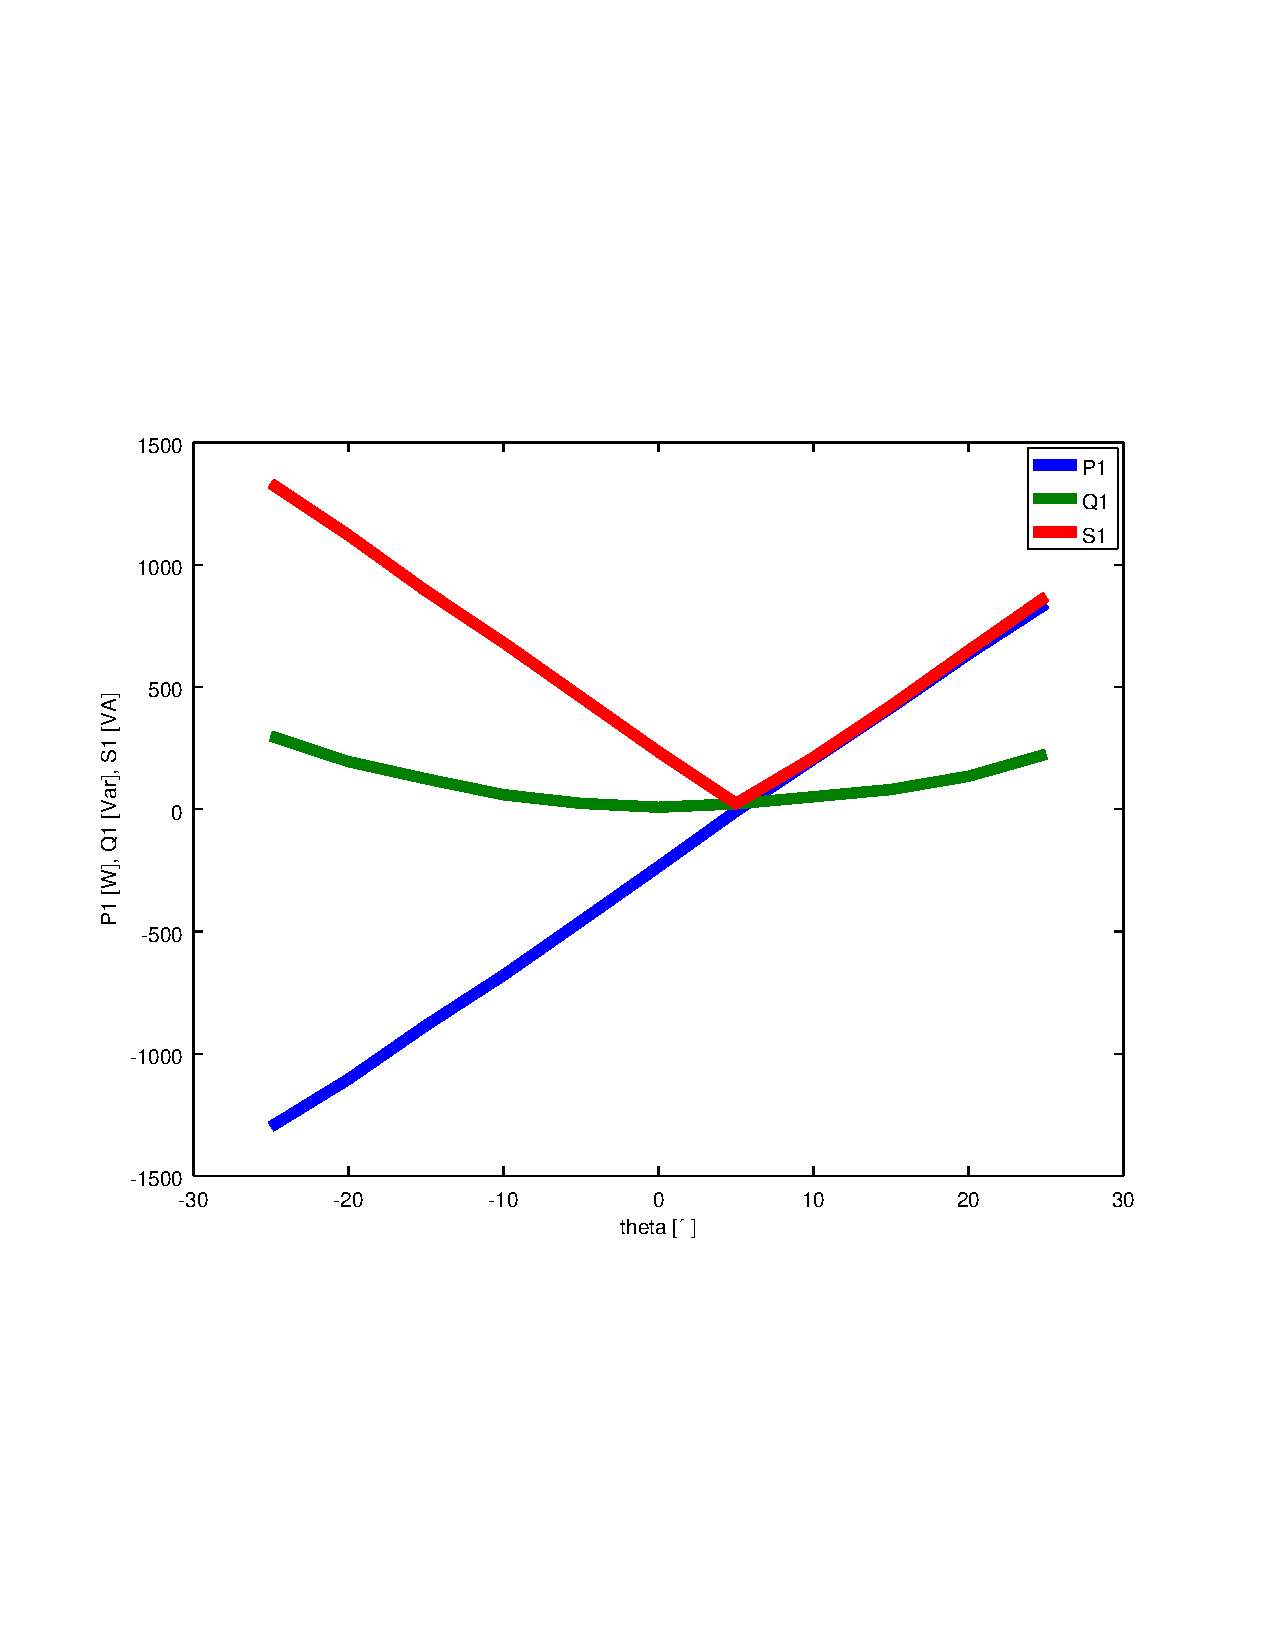
\includegraphics[width=0.5\textwidth, trim={1cm 6.5cm 2cm 7cm},clip]{pic/6_1_grundfrequenztaktung/6_1_2_einst_wirk_und_blindleistung/P1_Q1_S1.pdf}
  \caption{$P1(\theta) (blau), Q1(\theta) (grün), S1(\theta) (rot)$ von dem Effektivwert in Abhängigkeit des Zündwinkels}
  \label{fig:6_1_2_1}
  \end{center}
\end{figure}

Die folgenden zwei Abbildungen zeigen nochmals die Wirk- bzw. Blindleistung im direkten Vergleich.


\begin{figure}[H]
  \begin{center}
  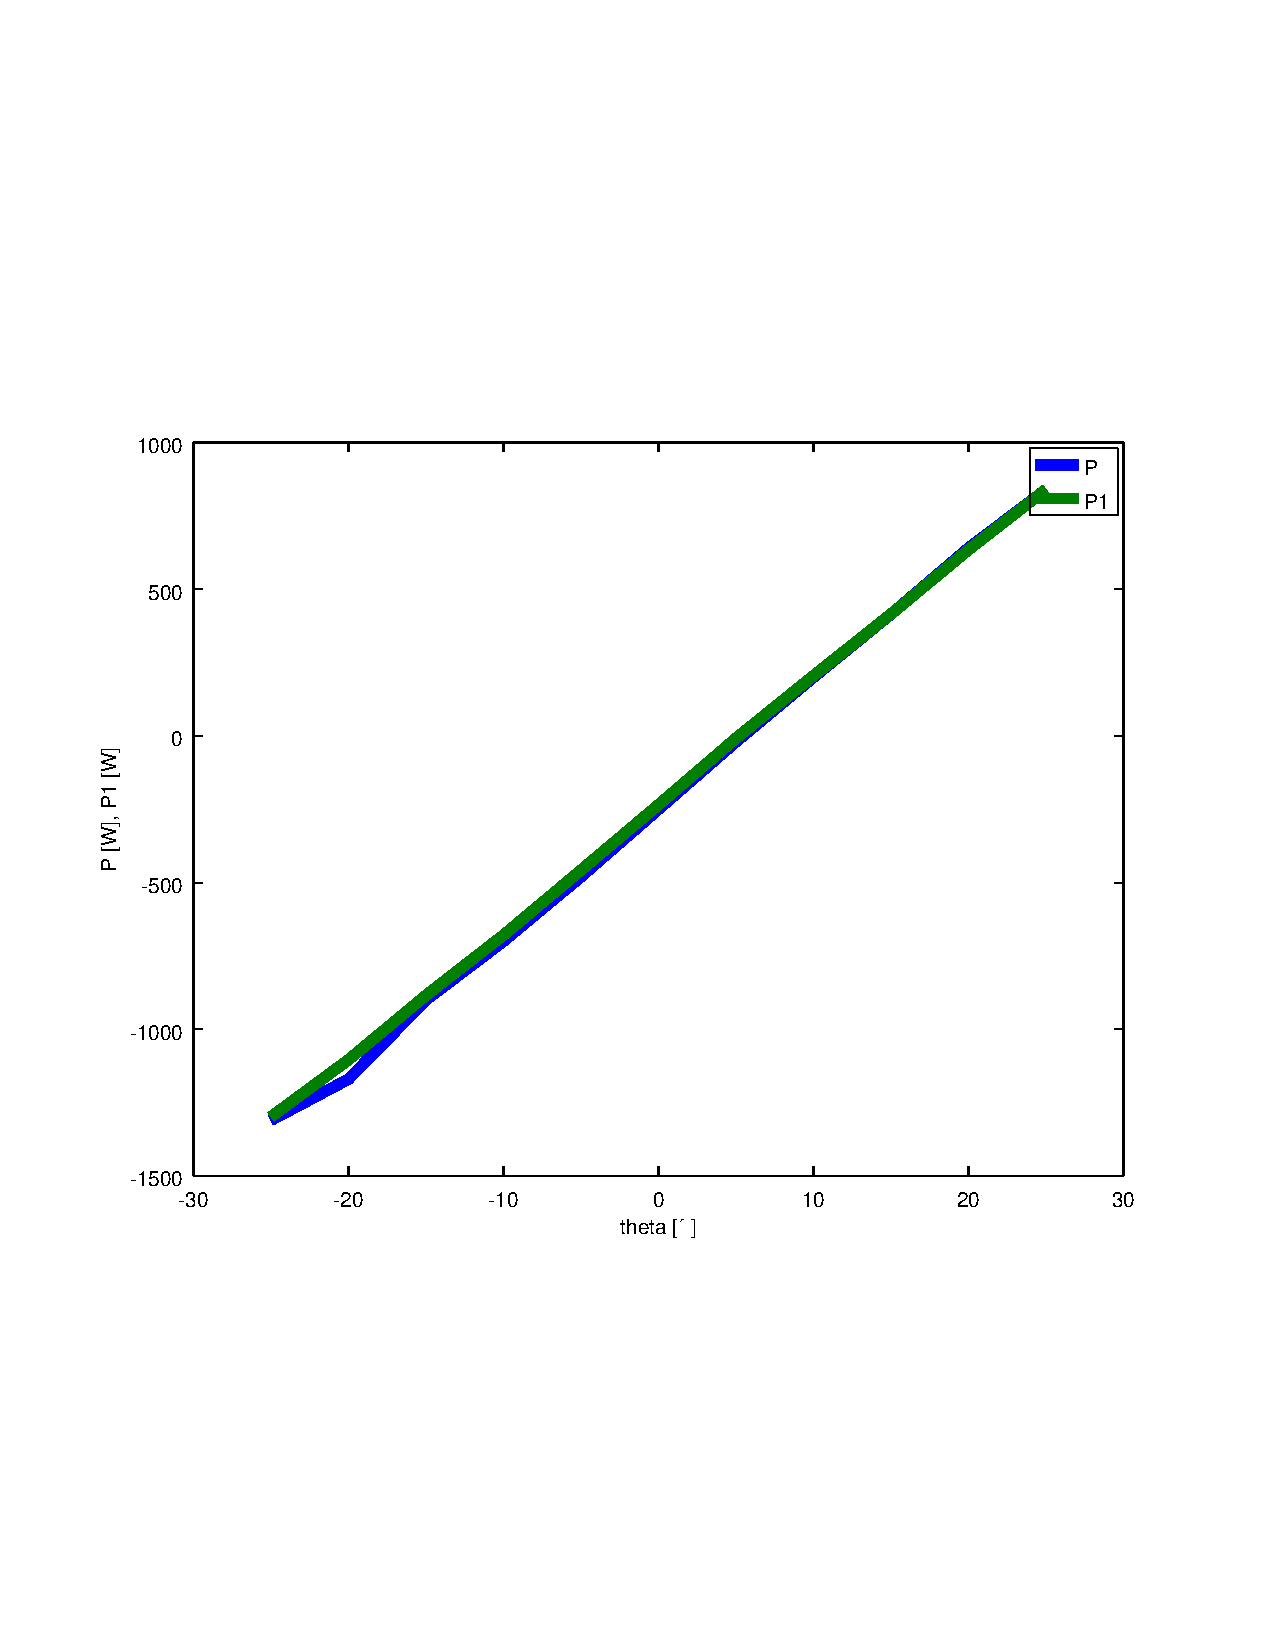
\includegraphics[width=0.5\textwidth, trim={1cm 6.5cm 2cm 7cm},clip]{pic/6_1_grundfrequenztaktung/6_1_2_einst_wirk_und_blindleistung/P_P1.pdf}
  \caption{Wirkleistung $P(\theta)(blau), P1(\theta) (grün)$ in Abhängigkeit des Zündwinkels}
  \label{fig:6_1_2_2}
  \end{center}
\end{figure}

Auffallend ist, dass beim Zündwinkel von $-30°$ die gesamte Wirkleistung kleiner ist als die der Grundschwingung. Eine mögliche Begründung wäre, dass in diesem Betriebspunkt die harmonischen Oberschwingungen zusätzlich Wirkleistung erzeugen und dies das Leistungsmessgerät beim Effektivwert nicht berücksichtigt.


\begin{figure}[H]
  \begin{center}
  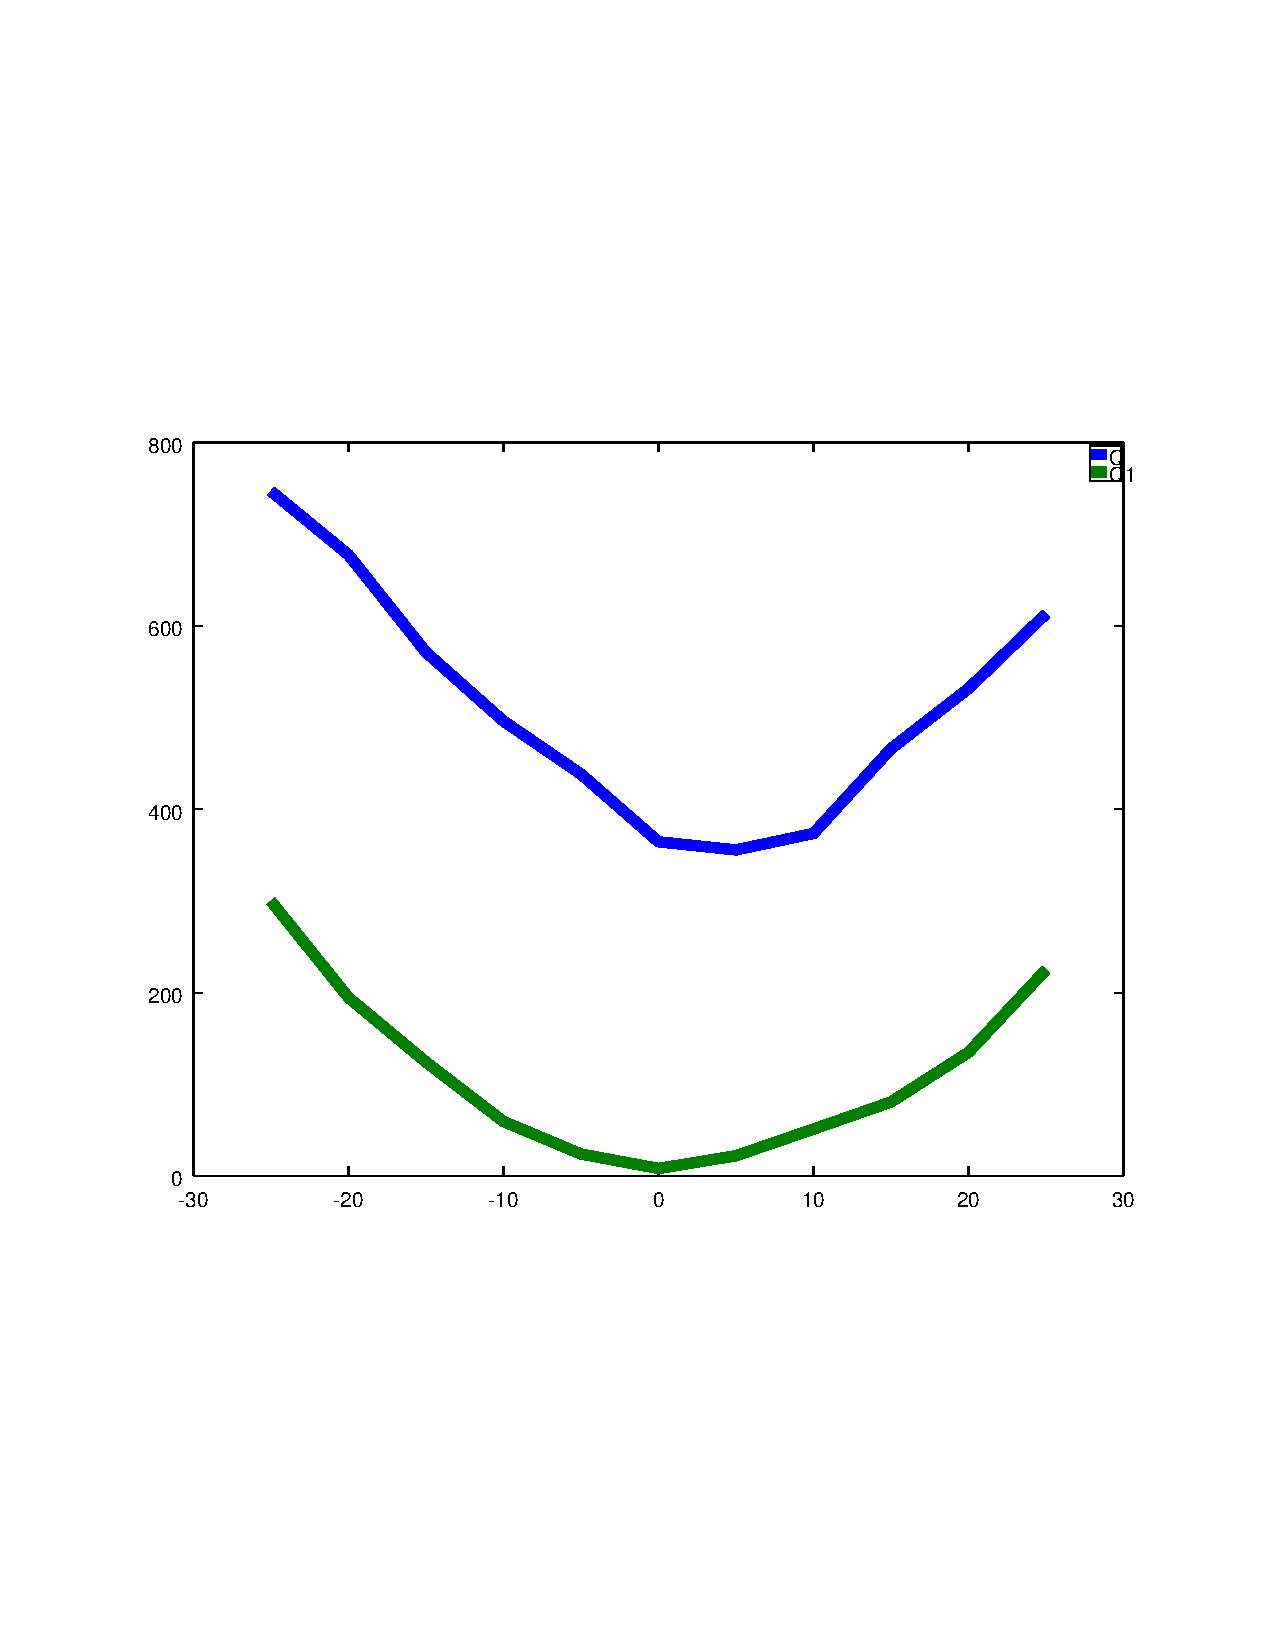
\includegraphics[width=0.5\textwidth, trim={1cm 6.5cm 2cm 7cm},clip]{pic/6_1_grundfrequenztaktung/6_1_2_einst_wirk_und_blindleistung/Q_Q1.pdf}
  \caption{Blindleistung $Q(\theta) (blau), Q1(\theta) (grün)$ in Abhängigkeit des Zündwinkels}
  \label{fig:6_1_2_3}
  \end{center}
\end{figure}
Die Blindleistung ist immer positiv da diese mit hilfe des Quadrats berechnet wurde.\\
Anhand der Abbildungen \ref{fig:6_1_2_0} - \ref{fig:6_1_2_3} ist zu sehen, dass der eingestellte Zündwinkel von $\theta = 5°$ dem effektiven Winkel von $0°$ entspricht. Denn in diesem Punkt gibt der Wechselrichter weder Wirkleistung ab noch bezieht er Wirkleistung.\\

Die Abbildungen \ref{fig:6_1_2_4} und \ref{fig:6_1_2_5} zeigen die Wirk- bzw. Blindleistung in Abhängigkeit von der Gleichspannung. Bei 310 Volt war der Wechselrichter synchron und der eingestellte Zündwinkel betrug $0°$.\\

$S = U * I$
I und P abgelesen
$Q = sqrt{S^2 - P^2}$

\begin{figure}[H]
  \begin{center}
  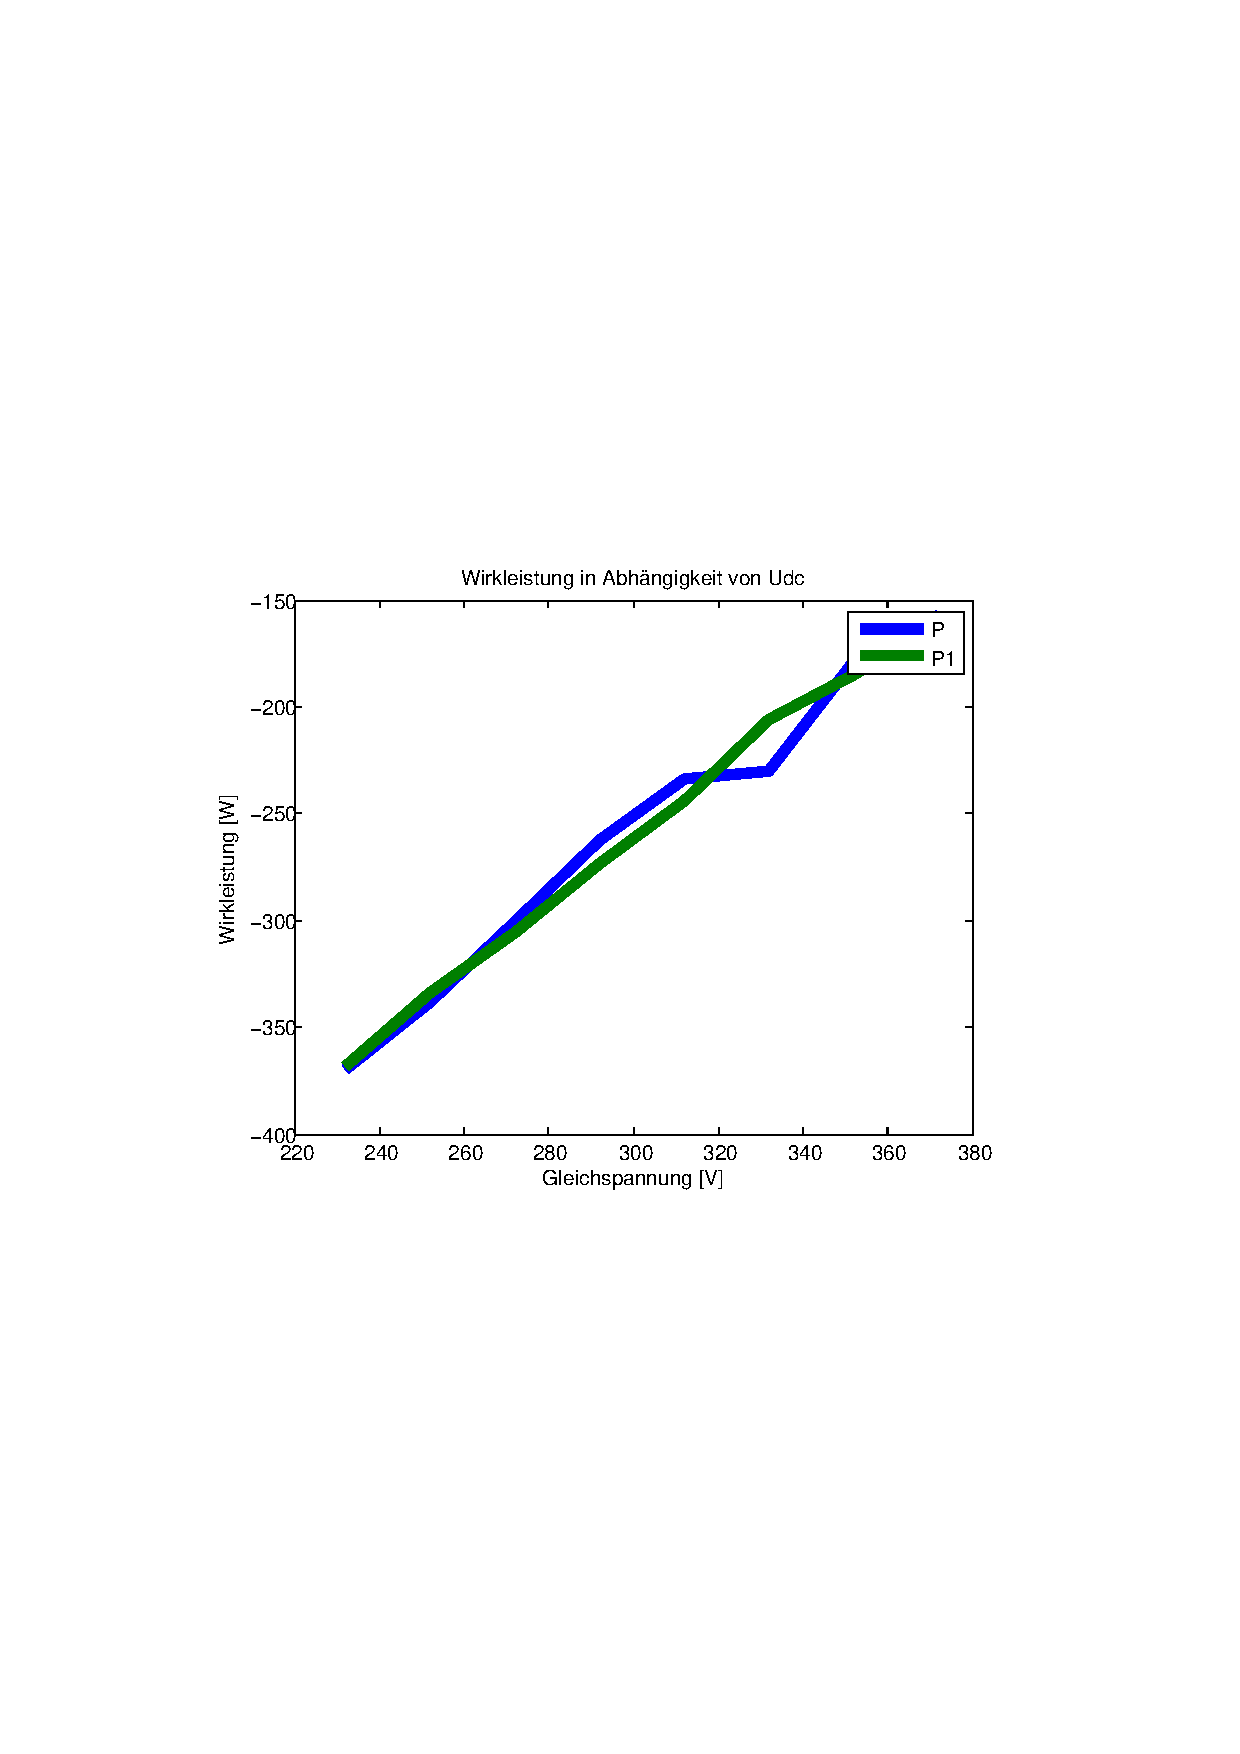
\includegraphics[width=0.5\textwidth, trim={1cm 6.5cm 2cm 7cm},clip]{pic/6_1_grundfrequenztaktung/6_1_2_einst_wirk_und_blindleistung/P_P1_Udc.pdf}
  \caption{Blindleistung $P(U_{DC}) (blau), P1(U_{DC}) (grün)$ in Abhängigkeit der Gleichspannung}
  \label{fig:6_1_2_4}
  \end{center}
\end{figure}


\begin{figure}[H]
  \begin{center}
  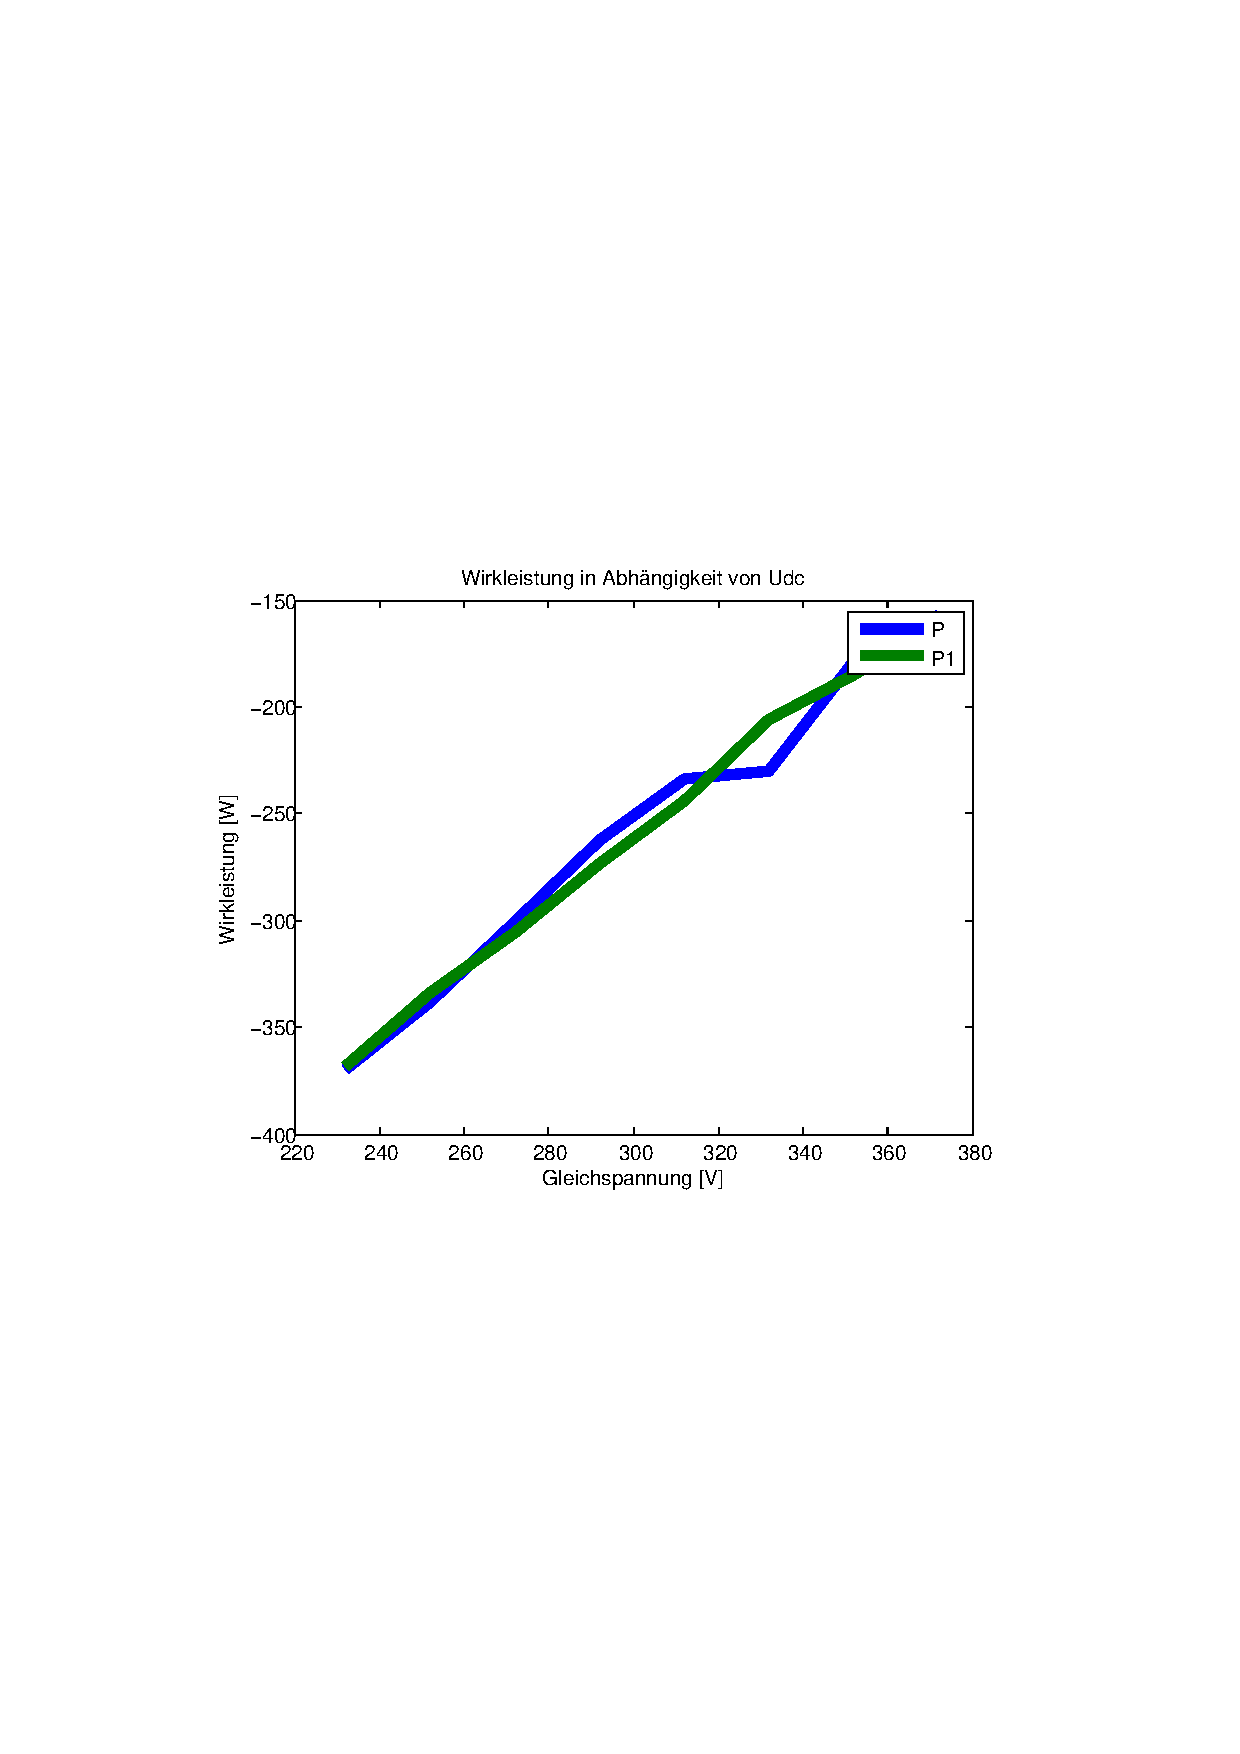
\includegraphics[width=0.5\textwidth, trim={1cm 6.5cm 2cm 7cm},clip]{pic/6_1_grundfrequenztaktung/6_1_2_einst_wirk_und_blindleistung/P_P1_Udc.pdf}
  \caption{Blindleistung $Q(U_{DC}) (blau), Q1(U_{DC}) (grün)$ in Abhängigkeit der Gleichspannung}
  \label{fig:6_1_2_5}
  \end{center}
\end{figure}

\clearpage